\documentclass[10pt,twocolumn]{article}
\usepackage{ipdps}
\usepackage{times}%
\usepackage{epsfig}%

\usepackage{vmargin}%
\usepackage{nopageno}
\setpapersize{USletter} %
\setmargnohf{0.8125in}{1in}{6.875in}{8.875in}

\setlength{\footskip}{0.6in}

\makeatletter \long\def\unmarkedfootnote#1{{\long\def\@makefntext##1{##1}
\footnotetext{#1}}} \makeatother

\pagestyle{plain}

\newenvironment{twoaffiliations}{\begin{tabular}{cc}}{\end{tabular}}
\newenvironment{oddaffiliation}{\centering}{\\~\\}

\newcommand{\superscript}[1]{\ensuremath{^\textrm{#1}}}
\newcommand{\subscript}[1]{\ensuremath{_\textrm{#1}}}

\graphicspath{{pdfplots/}}

\title{Performance Modelling of Peer-to-Peer Routing}

\author{
Idris A. Rai, Andrew Brampton, Andrew MacQuire and Laurent Mathy\\\\
Computing Department,\\
Lancaster University\\
\{rai,brampton,macquire,laurent\}@comp.lancs.ac.uk }

\begin{document}

\maketitle
\thispagestyle{empty}

\begin{abstract}
%Numerous peer-to-peer routing protocols have been proposed over recent years,
%yet almost all rely on simulation or implementation results for analysis. Very
%few such protocols have ever been mathematically modelled to formally prove
%their performance. In this paper, w
We propose several models based on discrete-time Markov chains for
the analysis of Distributed Hash Tables (DHTs). Specifically, we
examine the Pastry routing protocol, as well as a Stealth DHT
adaptation of Pastry to compute their exact expressions for average
number of lookup hops. We show that our analytical models match with
the protocols' simulation results almost perfectly, making them
ideal for rapid evaluation.
\end{abstract}

\unmarkedfootnote{\\1-4244-0910-1/07/\$20.00 $\copyright$2007 IEEE.}

\section{Introduction}
Peer-to-peer routing has now been used for several years in a diverse range of
applications. Despite the age of many such protocols, little work has gone into
providing their formalised models. Existing analysis typically consists of
simulated network scenarios rather than any proven mathematical models. While
this is not necessarily the case for older, unstructured algorithms, it is
certainly true for newer, structured protocols. As compared to simulations,
models can allow for much quicker evaluation of protocols at a wide range of
settings. Furthermore, they can sometimes help to gain an in-depth
understanding of the protocols. Given the popularity of many such peer-to-peer
systems, it is therefore important to provide their formalised models.

%Perhaps the most common form of structured, decentralised peer-to-peer protocol
%is the Distributed Hash Table (DHT), such as Pastry, Tapestry, Chord and
%CAN~\cite{Rowstron01Pastry, Zhao04Tapestry, Stoica01Chord, Ratnasamy01Scalable}.
%These systems aim to provide large-scale, distributed hash table functionality
%with the ability to \emph{put} and \emph{get} data indexed by hashed keys.
%Usually, this is achieved by randomly placing peers into a sparsely-populated
%overlay address space, and then assigning responsibility for a given index in
%the hash table to the node with the overlay address closest to the key. The
%randomness intrinsic to this approach aims to ensure that the data stored on
%each node is uniformly balanced across all nodes as well as balancing the load
%caused by messages sent within the overlay.

The approach to routing in most Distributed Hash Table (DHT) based peer-to-peer
systems involves iteratively or recursively forwarding a message closer to its
eventual destination based on local knowledge at each node, reducing the number
possible recipients with each hop. Consequently, most protocols (\emph{e.g.}
Pastry, Tapestry, Chord and CAN ~ \cite{Rowstron01Pastry, Zhao04Tapestry,
Stoica01Chord, Ratnasamy01Scalable}
%Kademlia~\cite{Maymounkov02Kademlia},and Viceroy~\cite{Malikh02Viceroy})
offer an expected $O(log N)$ number of lookup hops as an upper
bound.
% AB: Chopped this
%(CAN uses a degree $d$ to achieve an expected $O(dN^{1/d})$ hops).
In many of these previous works, this represents the extent to which
the proposed systems are mathematically modelled; all remaining study
is based upon simulation or implementation results.

In this paper, we aim to address the lack of formal DHT mathematical
analysis by modelling DHT  routing protocols using discrete-time
Markov chains to compute the expected number of lookup hops. Specifically, we consider the Pastry
protocol~\cite{Rowstron01Pastry} and a ``Stealth DHT'' adaptation of
Pastry~\cite{Brampton06Stealth}. As Pastry was one of the first DHT
protocols to be proposed, it provides a suitably general
representation of DHT routing that we also describe in greater
detail in Section~\ref{sect.pastry}. Conversely, our previously
proposed Stealth DHT work is a recent development, allowing for
unreliable nodes to be separated from core DHT routing at a low
cost, as explained further in Section~\ref{sect.stealth}.

We know of only one other work that mathematically analyses the performance of
DHT protocols~\cite{Spognardi06Formal}. This work proposes a formal framework
based on Markov chains to prove the performance of routing protocols in
BaRT~\cite{Spognardi02Bart} and Koorde~\cite{Kaashoek03Koorde}.
%Both are DHT-based routing
%protocols: BaRT is based on a randomised tree and
%Koorde is a Chord and de Bruijn graphs
%%~\cite{Bruijn46DeBruijn}
%based DHT.
Although the analytical approach taken by Spognardi \emph{et al.} also uses Markov
chains, the differences in routing methods between these protocols and Pastry
make it impossible to model Pastry and its associated Stealth DHT using the
exact methodology as proposed in~\cite{Spognardi06Formal}.

We first study \emph{Perfect Routing} models, wherein we assume that an
intermediate node along a routing path always finds the ``correct'' next hop
for a message. In practice, however, this is unrealistic; actual routing tables
are usually incomplete, with several empty cells. To counter this, we derive
other models for the protocols that emulate this imperfection: \emph{Models
with Imperfect Routing}. We define a route as ``failed'' if a node does not
forward a message via the next expected node
% AB: Maybe drop this for example, or generalise it to remove "prefix-match" discusion
(\emph{e.g.} it uses a entry that is closer to the destination but which shares
the same prefix-match length as itself with respect to the target ID). These
models allow us to derive the exact expressions for the number of average hops
required to reach any node in the DHT (\emph{i.e.} the lookup length).

We validate our models using simulations of the Pastry and Stealth DHT
protocols, finding that there is a good match between simulation results and
the models. Since simulations provide a realistic example of imperfect routing
tables, the good validation results show that the models formally prove the
routing performance of the protocols. Therefore, the expressions of the average
number of hops obtained through the models can be directly used instead of
simulations to quickly evaluate the protocols. Moreover, the model results show
that the increase in routing imperfection exponentially affect the lookup
length of the protocols. The results from the models also help to improve
understanding in the choice of Pastry's inherent configuration parameter $b$,
as defined in the following section.

The remainder of this paper is organized as follows: We present an
overview of Pastry in Section~\ref{sect.pastry}. In
Section~\ref{mod.pastry} we discuss the Pastry model with perfect
routing and derive the expressions for the average number of lookup
hops. We then discuss the Pastry model with imperfect routing and
validate the model using simulations in Section~\ref{mod.fpastry}.
We model Stealth DHT routing performance and validate the models in
Section~\ref{sect.stealth} before we finally conclude the paper in
Section~\ref{conc}.

%\section{Pastry}

\section{Pastry  Overview} \label{sect.pastry} Each node on a
Pastry network has a unique identifier (ID), randomly generated within the
address space. The address space is dynamically partitioned into regions with
each region being assigned to the single node whose ID is closest. Node IDs are
represented in base $2^b$ where $b$ is a constant representing the number of
bits in each digit of ID. Each node maintains a routing table, which is
conceptually a $log_{2^b}N \times 2^b$ array, where $N$ is the size of the
address space. Thus each row of the array is partitioned into $2^b$ cells,
which can accommodate more than one entry. The dimensions of the routing table
array are so given because the entries in a row~$n$ contain references to nodes
whose IDs share a common prefix of length $n$ digits. The first row is
conceptually row~$0$ containing entries that have no prefix match, and since
there are only $log_{2^b}N$ rows it is impossible to have all digits in common.

The routing procedure for a node that sends or forwards a message is to select
the row of its routing table corresponding to its prefix match with the
destination ID and pick as a next hop the entry of the column corresponding to
the value of the first (non-matching) digit of the destination ID. For example
if a message arrives and the destination ID has $n$ prefix matches, the next
node will be referenced in the $n^{th}$ row and in the $(n+1)^{th}$ digit's
column. This ensures that the next hop of the message shares a longer ID prefix
with the destination than the current node (and is therefore closer to the
destination).
% AB: Maybe the next sentence isn't important
% idris: no, we use this in stealth dht
It should be clear that one column per row of the routing table
contains an empty entry: this is the column corresponding to the $n^{th}$ digit
of the ID of the node holding the routing table (\emph{i.e.} the node itself).
This is because the corresponding entry in row $n$ would then share a prefix of
length $n+1$ with the node, and should therefore belong on the following row.
This very concise and simplified description of the routing procedure is
sufficient for our discussion and we refer the reader
to~\cite{Rowstron01Pastry} for further details of Pastry routing.

%\subsection{Average Performance Overview}
%
%\begin{figure}[tb] \centering
%     {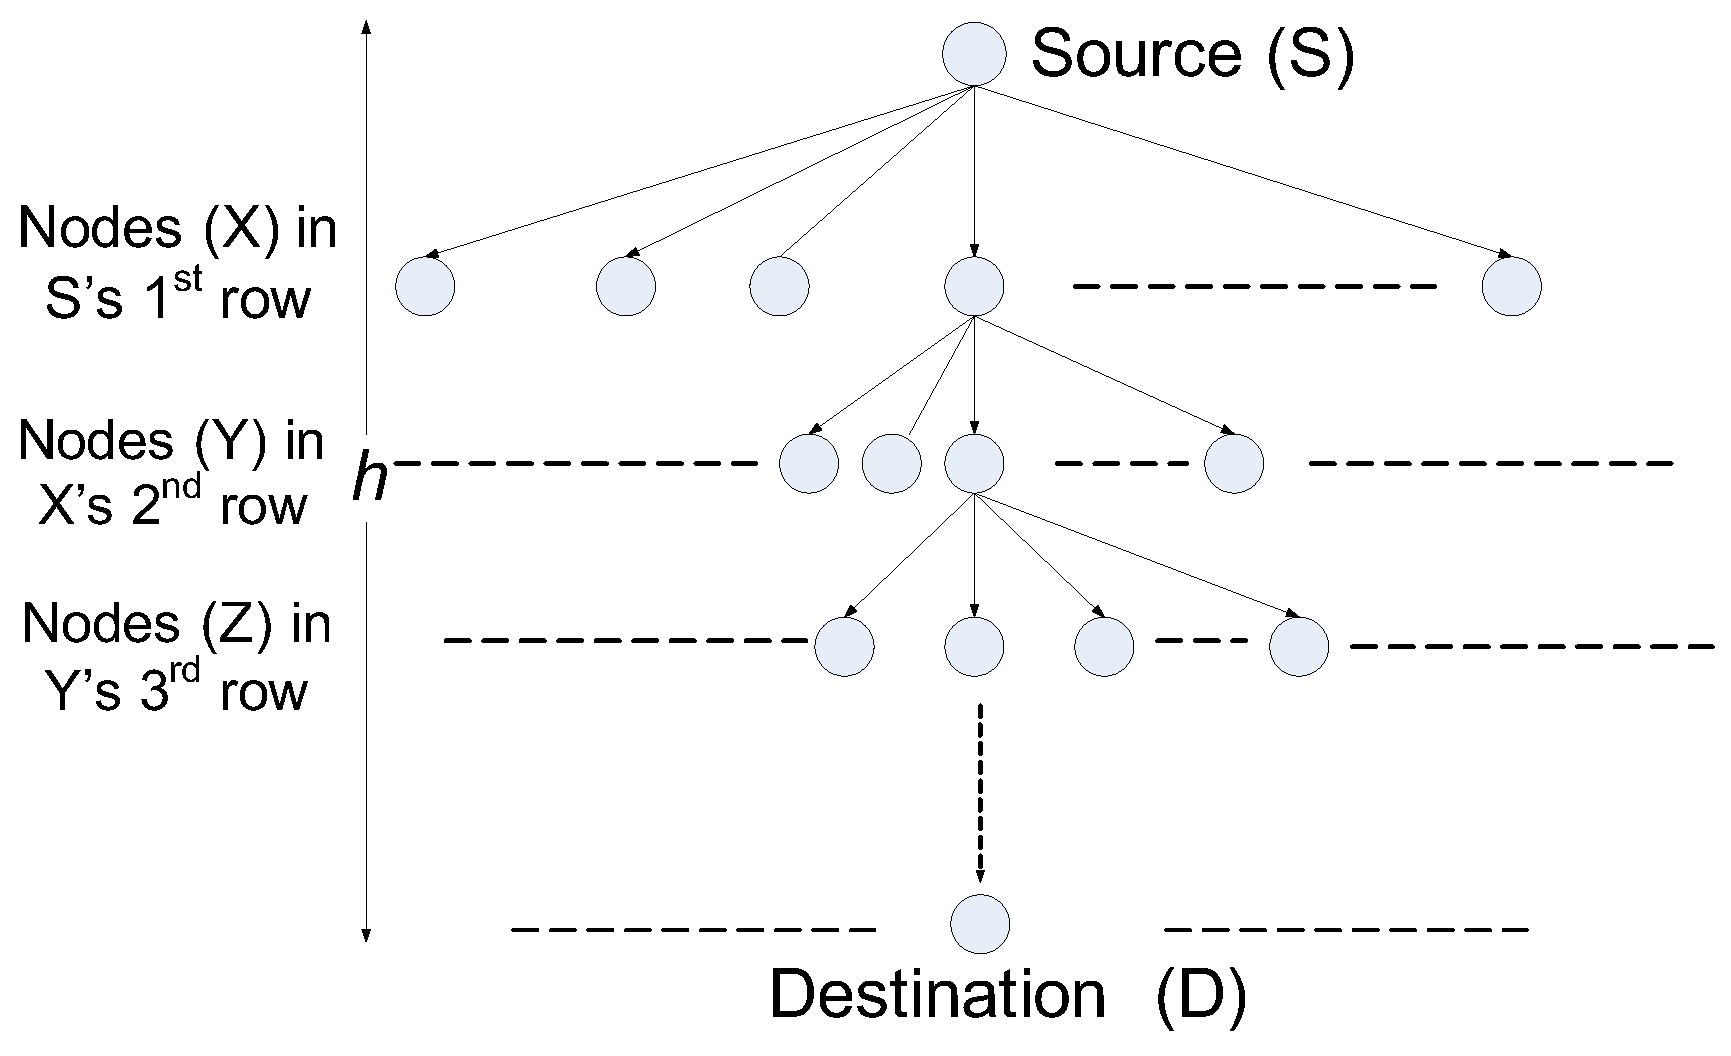
\includegraphics[width=0.35\textwidth]{Pastry-Tree}
%     \caption{2\superscript{b}-ary tree of Pastry routing tables}
%     \label{fig.pastry}}
%\end{figure}

The maximum number of hops per message for a Pastry network of $N$
nodes is given as $log_{2^b} N$. This expression is obtained
because, in Pastry, routing follows a path governed by a balanced
$2^b$-ary tree that spans the entire name space. The $2^b$-ary tree
is formed due to the structure of the routing tables, where each
node is a source for such a tree.
% as shown in Fig.~\ref{fig.pastry}.

In a $2^b$-ary tree, the network population is reduced by a factor
of $2^b$ each hop until the lookup message reaches the destination
node. The number of hops a message takes, $h$, is thus obtained as:
 $N/2^{(bh)}= 1$, which leads to  $h = log_{2^b} N$.

Therefore $h$ is the number of hops when each node along the path improves the
lookup path towards the destination by exactly one prefix match, which is an
ideal case. We call the expression $h$ the {\em Log Model} for
Pastry. In practice however, there is a chance of a node's ID improving the
match by more than one prefix, or a node may not improve the prefix match at
all (failed routes). In the former case, it is obvious to see that the actual
average number of hops per message in Pastry is less than $h$.

%\begin{figure}[tb] \centering
%     {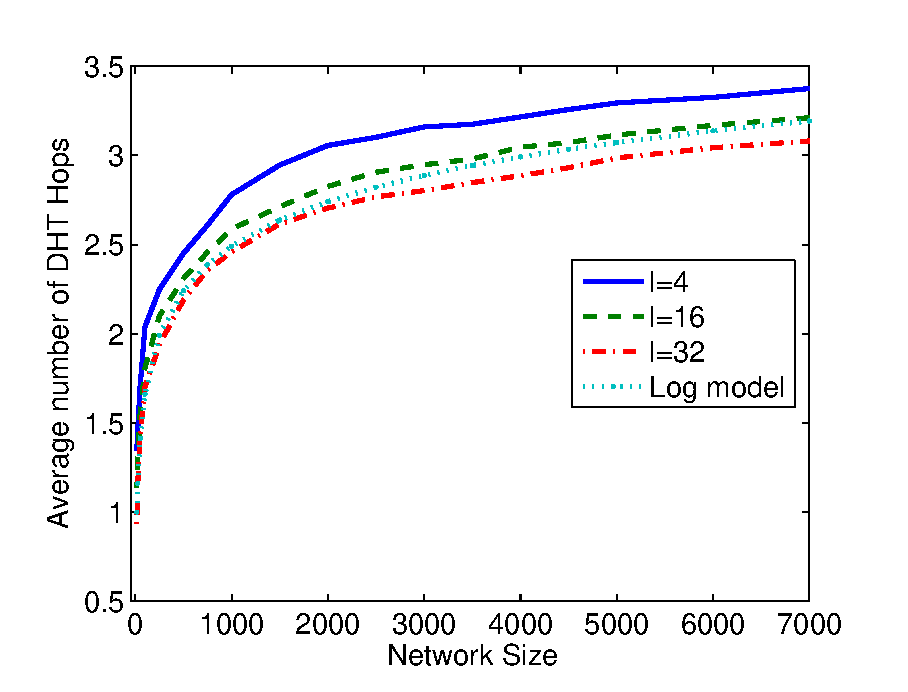
\includegraphics[width=0.35\textwidth]{pastry_vl}
%     \caption{Pastry routing  performance for varying leafset sizes}
%     \label{fig.pastry_val}}
%\end{figure}

Despite this, the Log model has been used to verify Pastry routing
performance before~\cite{Rowstron01Pastry, Brampton06Stealth}. We
found, however, that the use of the Log model to validate simulation
results depends on the input parameters used in simulators such as
leafset size. In this paper, we model Pastry and Stealth DHT routing
protocols to derive the exact expressions for the average number of
lookup hops.

%For example, we varied leafset sizes using $l = 4$, $l=16$, and $l =
%32$ (with $l=16$ and $l=32$ being recommended default values).
%Fig.~\ref{fig.pastry_val} shows the routing performance for
%simulation results for the considered leafset sizes and Log model.
%We clearly see that the model matches the simulation results well
%for the commonly used leafset size, $l = 16$.


\section{Pastry Model with Perfect Routing }
\label{mod.pastry}

In this section we consider an ideal Pastry routing protocol wherein a node
always forwards a message to the next hop that matches the key by at least one
prefix more than itself. Recall that an ID's digits are represented in
base~$2^b$. Therefore, the probability that  two randomly chosen IDs share a
single prefix is $p = 1/2^b$. Thus, the probability that two randomly chosen
IDs do not to share any prefix is $q = \frac{2^b - 1}{2^b}$.

A Pastry lookup (routing path) is made up of all nodes that participate to
deliver the message including the source and destination nodes. We model the
protocol using a discrete-time Markov chain where each state represents the number
of prefix matches a particular node shares with the destination. Each node on a
routing path is thus modelled by a state. Let $X_n$ be a state of the Markov
chain at a time $n$.  Pastry routing can be modelled using $h+2$ states such
that $X_n \in \{0,1,2, \cdots h, h+1\}$, where $h$ is the maximum number of
hops a message can take. A state $X_n = 0$ is also called the source state,
where a node has a key to lookup from the network. Conversely, state $X_n =
h+1$ is the destination state. Before sending a message, a source node may
already be at any state. For instance, it can be at state $h+1$ if its ID
matches that of the key, or at state $i$ if it shares $i-1$ prefixes with the
destination. At state $X_n=0$, a node only compares its ID to that of the key
to identify  the next node to forward the message to (the next state). At any
other state $i < h+1$, upon receiving a message to forward, a node finds the
next hop from its routing table.

The structure of routing tables, when they are full, guarantees each node on
the lookup path to improve the routing towards the destination by one prefix
match. In addition, nothing stops a node having more than one prefix match with
the target. This however, is not guaranteed and happens only by chance.
Therefore, the probability of improving a route by exactly one prefix match is
equal to the probability that the next digit following the guaranteed one in
the next hop ID does not match the corresponding digit of the destination ID.
From our previous discussion, this probability is $q$.

We denote transition probability from state $i$ to state $j$ as
$p_{ji}=P(X_n = j/X_{n-1}= i)$. From the routing discussion above,
we can see that transition probabilities  from state $i$ to state
$j$ ($p_{ji}$) always exist for all $j>i$. Note that $p{_{ji}}$ for
$j
> i+1$ represent transition probabilities when a node is fortunate enough to
improve the routing by more than one prefix match. The perfect
routing protocol ensures that a key gets closer to the destination
every time the message is relayed to another node, then for $j \le
i$, the conditional probability is:
\begin{equation}
 p_{ji} = 0 ~~~\forall j \le i
\end{equation}

Generally, a transition from state $i$ to state $j$ occurs when a node improves
the routing by $j-i$ prefixes, (\emph{i.e.}, the guaranteed prefix match and
$j-i-1$ extra matches that could happen by chance). Thus, the transition leads
to the following corresponding expression of transition probability:
\begin{equation}
\label{eq.1} p_{ji} = p^{j-i-1}q, ~~~~\forall j>i
\end{equation}
where $q=1-p$.

\begin{figure}[tb] \centering
     {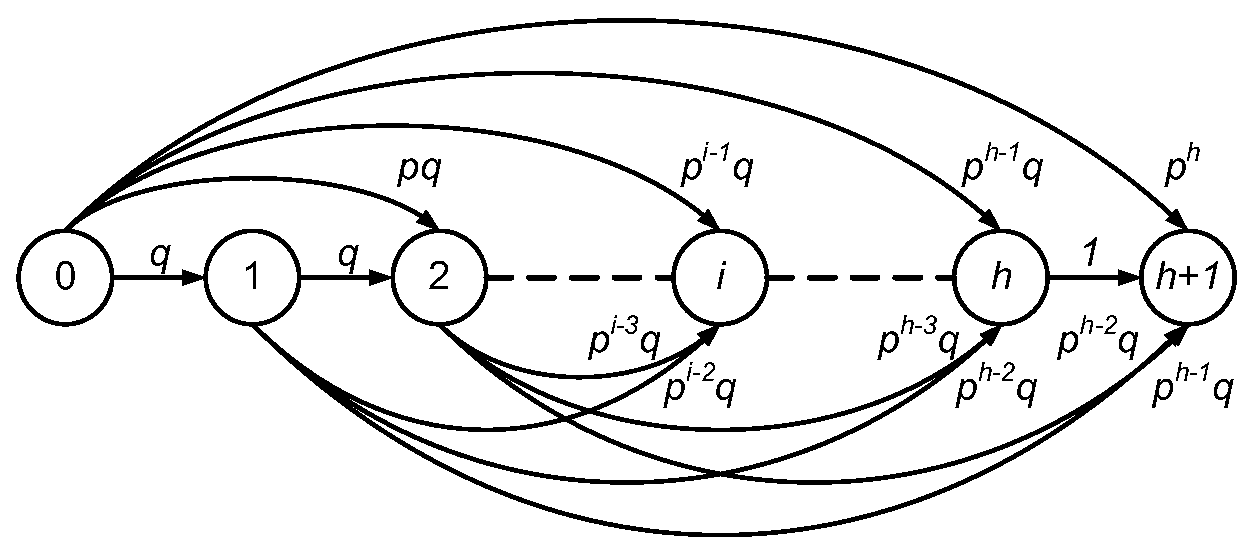
\includegraphics[width=0.35\textwidth]{Markov-NoFail.eps}
     \caption{Markov Chain without failures}
     \label{fig.mkv1}}
\end{figure}

Recall that the perfect routing model assumes that nodes and routes do not
fail, which means that $p_{jj} =0$. This allows us to get the general
expression for transition probabilities as follows:

\[ p_{ji} = \left\{ \begin{array}{ll}
         0 & \mbox{if $j \le i$}\\
         p^{j-i-1}q & \mbox{if $i < j \le h$} \\
         1   &  \mbox{if $i = h$, $j=h+1$}
         .\end{array} \right. \]
Fig.~\ref{fig.mkv1} shows the Markov chain for the perfect Pastry routing
model. Observing the figure, one can note that all states of the chain are {\em
transient} except the last state, which is absorbing since once entered, the chain
never leaves it. As a result, the
chain does not exhibit irreducible  and aperiodic properties necessary to
obtain steady state, stationary distributions. Therefore, the average number of
lookup hops, which is obtained from the mean recurrence time of state $h+1$,
cannot be computed from the Markov chain. To be able to derive the average
number of lookup hops, we transform the chain to an irreducible and aperiodic
Markov chain by  adding a sure transition from state $h+1$ to state $0$ as seen
in Fig.~\ref{fig.ergo}.

\begin{figure}[tb] \centering
     {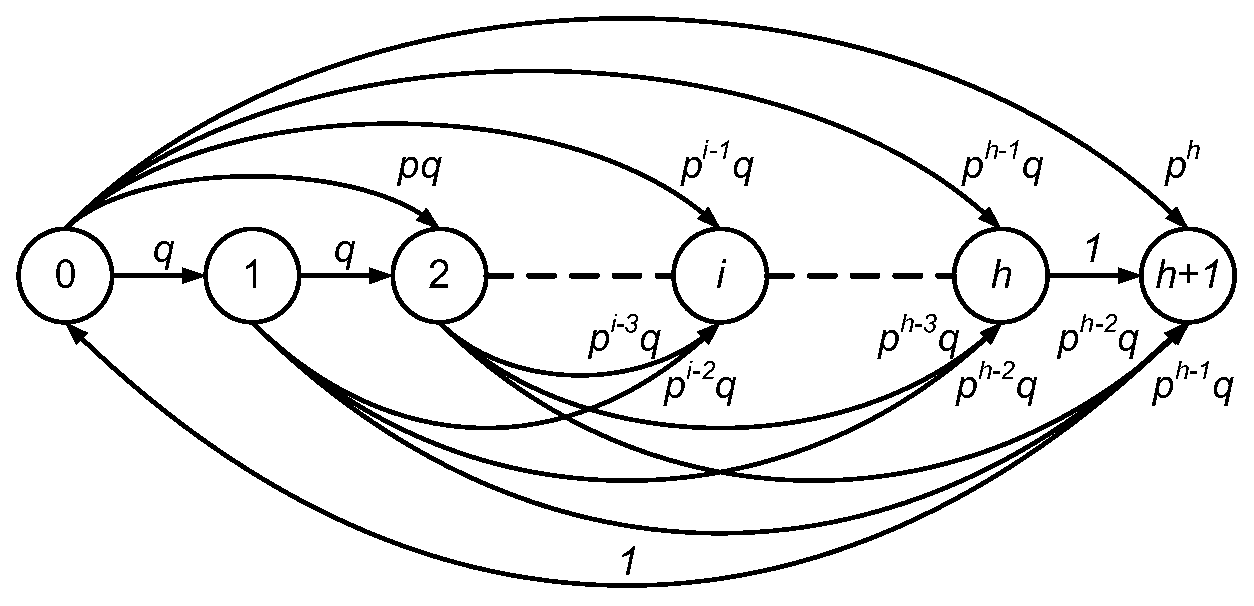
\includegraphics[width=0.35\textwidth]{Markov-Modify.eps}
     \caption{Modified Markov Chain for Pastry routing without failures}
     \label{fig.ergo}}
\end{figure}

The transition probability matrix for the Pastry routing model
corresponding to Fig.~\ref{fig.ergo} is:
\[ {\bf P} = \left( \begin{array}{ccccccc}
0 & q & pq & p^2q & \cdots  &p^{h-1}q & p^h  \\
0 & 0 & q & pq & \cdots &p^{h-2}q & p^{h-1}\\
0 & 0 & 0 &q & \cdots & p^{h-3}q & p^{h-2} \\
\cdots & \cdots & \cdots &\cdots & \cdots & \cdots & \cdots \\
0 & 0 & 0 &0 & \cdots & q & p \\
0 & 0 & 0 &0 & \cdots & 0 & 1 \\
1 & 0 & 0 &0 & \cdots & 0 & 0  \end{array} \right)\]

%AM: being picky, this sentence is a little awkward ('is' with singular then plural)

The solution of the chain, which is the steady state probabilities, is the
normalised solution of the following system of linearly dependent equations
with variable vector ${\bf x} = (x_0, x_1, \cdots,x_{h+1})$
\begin{equation}
\nonumber {\bf xP} = {\bf x}
\end{equation}

% AB: Can we put all these equations together and reference them, it would save some space
After some simple arithmetic operations and inspection of the transition
matrix, it can be shown that the solution to the above system of linear
equations is given as:
\[x_i = \left\{ \begin{array}{ll}
         x_{h+1}  & \mbox{if $i = 0$}\\
         qx_0  & \mbox{if $i = 1$} \\
         x_{i-1}  & \mbox{if  $1 < i \le h$} \end{array} \right. \]
The solution of the system is then given as
\begin{equation}
\nonumber \pi_i = \frac{x_i}{\sum_{j=0}^{h+1}{x_j}}, \mbox{for $0 \le i \le
h+1$}.
\end{equation}
It can be easily shown that
\begin{equation}
\nonumber \sum_{i=0}^{h+1}x_i = 2x_0 + hqx_0
\end{equation}
which implies that
\begin{equation}
\nonumber
 \pi_{h+1} = \frac{1}{2+hq}
\end{equation}

From Leon-Garcia~\cite{Garcia94Probability}, the mean recurrence time for state
$h+1$ is given as:
\begin{eqnarray}
\nonumber
E[T_{h+1}] &=& \frac{1}{\pi_{h+1}}\\
\nonumber
         &=& 2+hq
\end{eqnarray}
The average number of hops for a lookup to reach a destination is the average
number of transitions to move state $0$ to state $h+1$, which is equivalent to
the mean recurrence time of state $h+1$ minus the transitions that do not
represent hops, \emph{i.e.}, from state 0 to all other states and from state
$h+1$ to state 0. Recall that transitions from state $0$ are not hops as they
only represent a {\em chance} prefix match the source may have with the target,
and the transition from state $h$ to state $0$ does not represent a hop and is
added only  to obtain stationary probabilities of the Markov chain. The
aggregate expected probability for these two cases of transitions is equivalent
to $\sum_{i=1}^{h+1}p_{i0} + p_{0,h+1}$, which is 2. We therefore obtain the
average number of hops for Pastry with perfect routing ($H_{pastry}$) as
follows:
\begin{eqnarray}
\nonumber
H_{pastry} &=& E[T_{h+1}] - 2 \\
\label{eqn.pastr}
  &=& hq
\end{eqnarray}

Note that the comparison between the average routing performance of
the Pastry model with perfect routing (Equation (\ref{eqn.pastr}))
and the Log model ($log_{2^b} N$) is a function of $q$, which is a
protocol configuration parameter $b$. The value of $b=4$ has been
typically used in Pastry~\cite{Rowstron01Pastry}. Using the derived
expression for the average number of hops, we can determine  how the
performance difference between the Log model and the Pastry model
depends on $b$ values. Particularly, the ratio of the average number
of hops of the Log model and the Pastry model without failures is
$1/q = \frac{1}{(1-1/2^b)}$. Note that  $lim_{b\rightarrow \infty}
1/q \rightarrow 1$, which means that the model asymptotically
converges quickly to the upper bound. This shows the extent to which
the average number of hops between the two models compares as $b$
varies, which can aid in deciding on an appropriate value of $b$.
From this, we can conclude that small values of $b$ are the superior
options.

\subsection{Validation}
We validate our  models against simulations that were carried out
using our own discrete-event packet-level Pastry simulator, based on
Pastry~\cite{Rowstron01Pastry}. In~\cite{Brampton06Stealth}, we
showed that our simulator can be  validated  against Microsoft's
Pastry Version 3.0A simulator, as well as a real world
implementation. Each network size was simulated at least five times
on a famous GT-ITM~\cite{Calvert97Modeling} generated transit-stub
topology of 1,000 routers, with 4\% transit nodes. DHT nodes, whose
numbers we vary from 10 to 7,000, were connected to this topology in
a random fashion. In each simulation run, 10,000 messages (each with
a randomly generated key) were sent from a randomly selected source.

\begin{figure}[tb] \centering
     {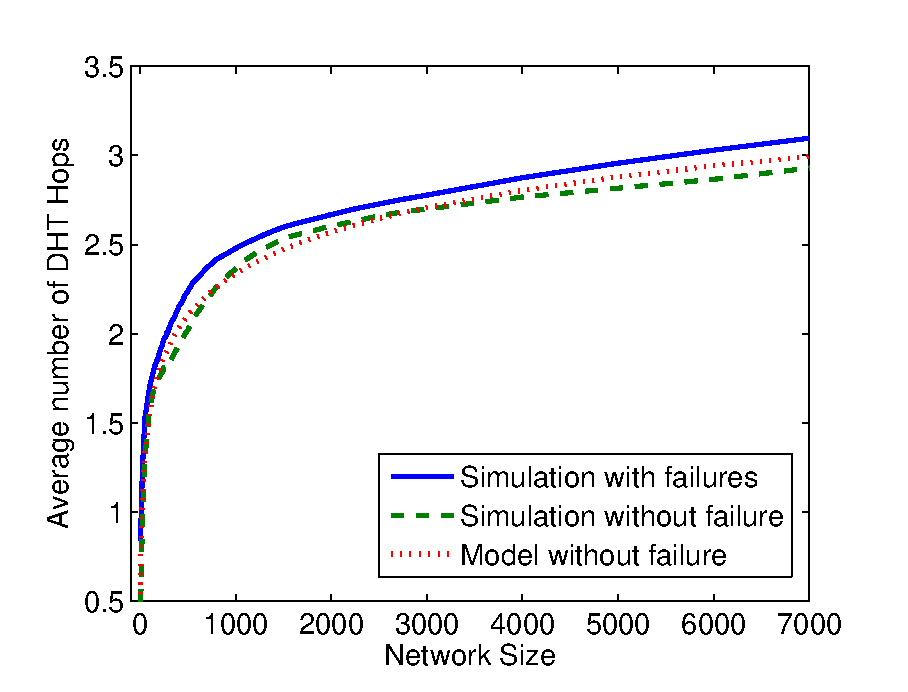
\includegraphics[width=0.35\textwidth]{val_past1.eps}
     \caption{Validation of Pastry model without routing failures}
     \label{fig.valid1}}
\end{figure}

Fig.~\ref{fig.valid1} shows the average number of hops for the perfect routing
model and for the simulations, both with and without failures. The latter is
obtained by considering only messages that were delivered without routing
failures. We clearly see that the results for the Pastry model with perfect
routing matches well against the simulation results of Pastry without failures.
However, the model underestimates the simulation results with failures.
%Note
%also that the Log model, not shown in the figure, would not match the
%simulation without failures since (as also seen in Figure~\ref{fig.pastry_val})
%it always matches simulation results with routing failures for $l=16$, which is
%the value used for these simulations.

By definition, the perfect routing model assumes that no route between nodes
fails. That is, a node in the perfect routing model always finds the correct
next hop reference in its routing table, which is possible only if routing
tables are full. Full routing tables further imply
that all nodes along a routing path use their routing tables to identify the
next hop (except the node just before the destination). However, note that
$p_{{h+1},{h}} =1$ indicates that the next hop for the last hop can either be
determined using routing tables or leafsets.

Realistically, available routing table population mechanisms in Pastry do not
guarantee complete routing tables, and neither is this required for the
protocol to work. It is often the case that some cells in a routing table are
empty.  We therefore next model Pastry routing performance taking into account
this routing imperfection.

\section{Pastry model with imperfect routing}
\label{mod.fpastry} We say a route between two nodes fails if a node finds that
the cell for the expected correct reference to the next hop is empty. When a
route fails, a forwarding node has to look for another next hop reference from
other cells in its routing table. The new next hop reference is often chosen as
the closest node to the destination on the same row of the routing table as the
missing entry. Therefore, it does not improve the lookup towards the
destination because, except for the entries in the correct cell, all entries on
the same row share the same number of prefixes to the key as the node holding
the routing table. From a Markov-chain perspective, this means that the state
of the chain is unchanged. The same applies if the failed route occurs at the
source of the message.

\begin{figure}[tb] \centering
     {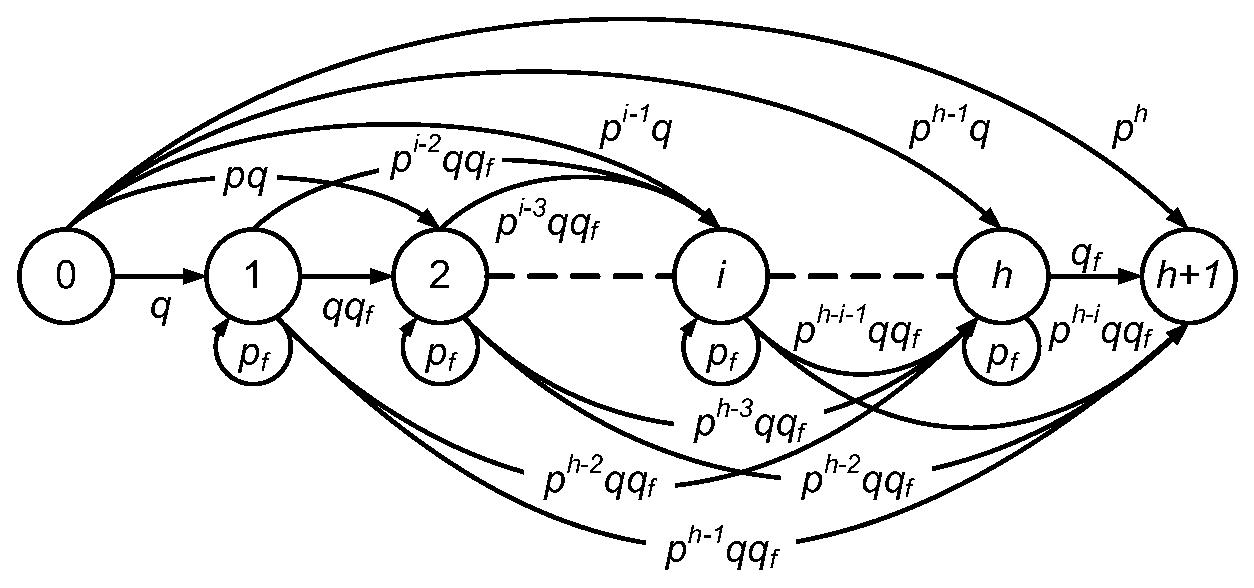
\includegraphics[width=0.35\textwidth]{Markov-WithFail.eps}
     \caption{Markov Chain with routing failures}
     \label{fig.mkv2}}
\end{figure}

We assume that a message is equally likely to fail at any state with
probability $p_f$. Transition probabilities for the model with failures are
obtained in a similar way as the model without failures and are summarised as
follows:

\[ p_{ji} = \left\{ \begin{array}{ll}
         0 & \mbox{if $j < i$}\\
         p_f & \mbox{if $j = i$,  $i \neq 0, h+1 $}\\
         p^{j-i-1}q & \mbox{if $i = 0$, $\forall~~j>i $} \\
         p^{j-i-1}qq_f & \mbox{if $i \ge 1$, $i < j \le h$} \\
         q_f & \mbox{if $i = h$, $j = h+1$}
         .\end{array} \right. \]

Fig.~\ref{fig.mkv2} shows the Markov chain for the model. Note that routes do
not fail at states $0$ and $h+1$. Recall that state $0$ is the state used to
decide the source's beginning state on the chain, and state $h+1$ is the
destination.

Using the same procedures as used for the Pastry model with perfect
routing, we obtain the average number of lookup hops for Pastry
routing model with failures as:
\begin{eqnarray}
H^f_{pastry} &=& h\frac{q}{q_f}
\end{eqnarray}
where $p_f$ is the probability of route failure and $q_f = 1-p_f$.
We next discuss validation results of the model using simulations of
the protocols.

\begin{figure}[tb] \centering
     {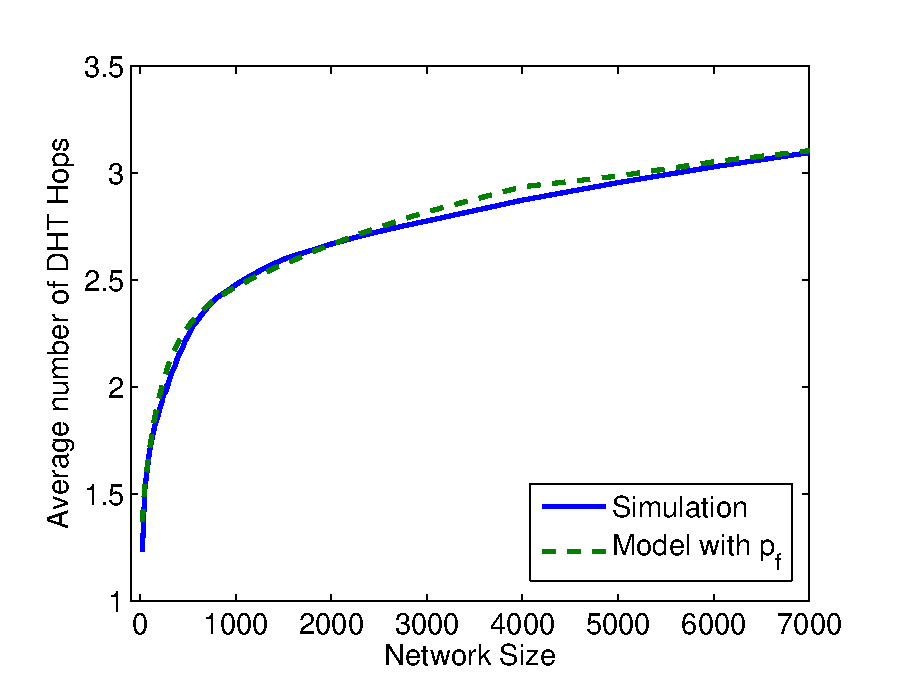
\includegraphics[width=0.4\textwidth]{val_past2.eps}
     \caption{Validation of Pastry model with routing failures}
     \label{fig.valid2}}
\end{figure}

\subsection{Validation}
% AM: are we implying we're not using the correct approach?
Before presenting the validation results, we first discuss the various methods
we used to compute the probability of route failures. The correct approach is
to analytically compute the probability of failures based on network input
workload. As our efforts in this regard proved futile, we resorted to the use
of simulation results. There are two possible ways this can be done: one is to
use the fraction of empty cells per row in a routing table, the other involves
tracking down all hops that are due to failed routes. We considered the latter
option over the former as it provides the actual failures from the simulation.
As such, we tracked all instances in the simulator whereby a node fails to find
a next hop reference in its routing table. If we denote the number of failed
routes from the simulations, the total number of messages, and the average
number of hops for simulations as $F_r$, $M$, and $H_{sim}$ respectively, then,
for each network size, we compute the probability of route failure per state
as:
\begin{equation}
\label{rf} p_f = \frac{F_r}{H_{sim}M h}
\end{equation}
Where $h$ is the number of states where route failures are possible. In some
cases a fixed probability ($\overline{p_f}$) of route failure per state for
each network size computed as the mean of probabilities obtained from
simulations as given in Equation~(\ref{rf}) offers good validation results.

Fig.~\ref{fig.valid2} shows the average number of hops for the model against
the simulation results  as a function of network size. We observe that
simulations match the results of the model very well when $p_f$ as given in
Equation~(\ref{rf}) is used.

\begin{figure}[tb] \centering
     {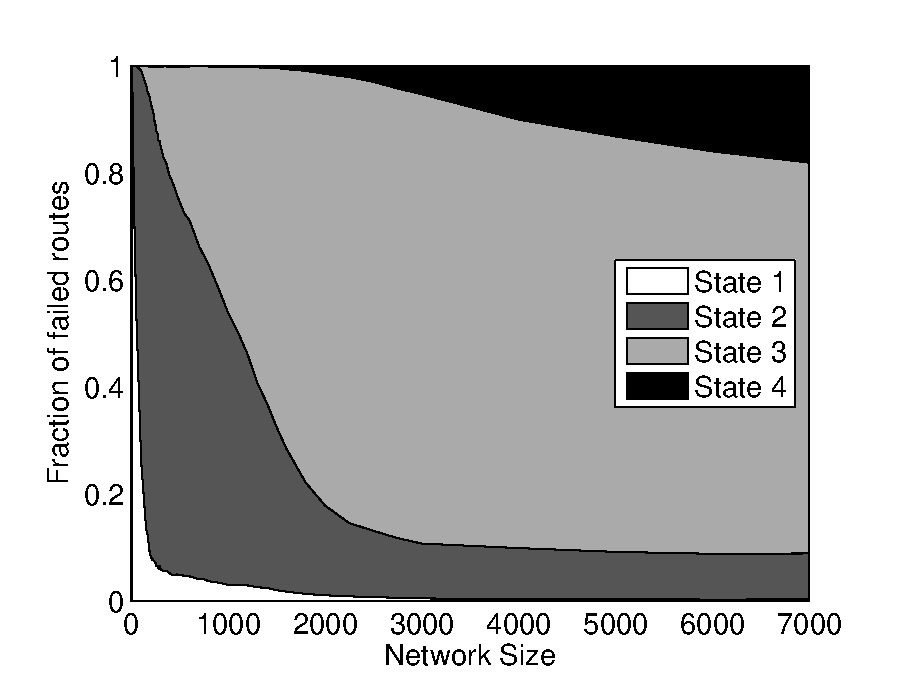
\includegraphics[width=0.4\textwidth]{prob01.eps}
     \caption{The Distribution of route failures as a function of states}
     \label{fig.fm}}
\end{figure}

It should be noted that both approaches of computing the probability of route
failure per state result in some  estimation of failure probabilities only.
Moreover, the assumption that the probability of a route failure is the same
for each hop is not realistic. Simulation results show that a large fraction of
route failures occur at a single state. To illustrate this, Fig.~\ref{fig.fm}
shows the distribution of route failures  at different states for varying
network sizes. It can be
observed from the figure that, for a given network size, the majority of
failures occur at a single state, and that this concentration changes depending
on the size of the network. For example the percentage of route failures for a
network of 3,000 nodes are $<$1\%, 10\%, 83\% and 5\% for states 1, 2, 3 and 4
respectively. Therefore, route failure is not uniform along the states. Despite
the mentioned approximations, the validation results in Fig.~\ref{fig.valid2}
show that the model matches well with the simulations.

\section{Stealth DHT}
\label{sect.stealth}
\subsection{Preliminary background}
We previously proposed the Stealth DHT concept to mitigate several performance
and security issues encountered in existing DHTs~\cite{Brampton06Stealth}. A Stealth
 DHT implementation
of a given DHT algorithm creates two distinct sets of nodes with differing
routing properties on the same overlay, namely \emph{Service} and
\emph{Stealth} nodes. Service nodes provide the routing infrastructure for the
overlay, whereas stealth nodes communicate with and through service nodes only.

The join process for most DHT implementations involves a node first gathering
state. Usually, this is achieved by routing a join message addressed to its own
ID into the DHT via a bootstrap node\footnote{An already-connected node
discovered through some alternate mechanism}. Nodes along the message's path
then reply directly with relevant routing information for the joining node.
Once the joining node receives notification that its message has reached its
destination, it announces its presence on the network so that other nodes may
route messages through it. Stealth DHTs achieve the separation of nodes by
halting the join process for stealth nodes after they have gathered state, but
before they announce their presence on the DHT. The resultant effect is that
stealth nodes do not appear in any routing tables, and thus are not used to
forward any messages or store any keys.

Stealth nodes only initiate routing of messages by selecting the first hop.
Therefore, they do not need to maintain a leafset which is only used to
consistently determine the last hop. Stealth nodes maintain a pruned version of
a routing table with only one row. This is deemed enough and has a negligible
negative impact on routing performance while significantly, reducing overhead.
This is because stealth nodes are only the origin of any messages they send
through the DHT.

Since stealth nodes have a reduced routing table, all cells in its single row
should be populated with appropriate entries. This ensures that a complete and
valid routing table at a stealth node will always provide a next hop that has
at least a one-digit prefix-match with the destination.

\subsection{Modelling Stealth DHT}
From the service nodes' perspective, the same model as for Pastry applies. That
is, the average number of hops a lookup takes is the same as in a Pastry DHT
with the network population comprised only of service nodes. In this section
therefore, we need only derive the average routing performance for stealth
nodes. We first derive models when only stealth nodes are considered as the
origins of messages, and then present the expressions for the average number of
lookup hops for the Stealth DHT with all nodes sending messages.

Observe that the first hop a stealth node makes is similar to the first hop of
a service node which uses the first row of its routing table. Thus, the maximum
number of lookup hops is the same as just considering a population of only
service nodes. To clarify: let the fraction of service nodes be $r$ and $N$ the
total number of nodes in the network, then for a Stealth DHT, $h = log_{2^b}
rN$.

\subsection{Perfect Routing Model}
A stealth node does not need to compare its own ID to the target key, instead,
it immediately selects an appropriate node to send the message to from its
routing table. Indeed, even if the stealth node does share an initial prefix
match with the key, its routing table will not enable a transition to any state
from state $0$ other than state $1$ since it has only one row in its routing
table. Therefore, the transition probability from state $0$ is given as:
\[p_{i0} = \left\{ \begin{array}{ll}
         0 & \mbox{if $i > 1$}\\
         1 & \mbox{if $i = 1$}
         .\end{array} \right. \]
Unlike the models for a Pastry DHT, the transition from state 0 to state 1 in a
Stealth DHT therefore represents the fact that a stealth node always has to use
its first row of the routing table to send a message. This, together with the
modified value of $h$  for Stealth DHTs, are the main distinguishing points in
modelling a Stealth DHT from modelling Pastry.

\begin{figure}[tb] \centering
     {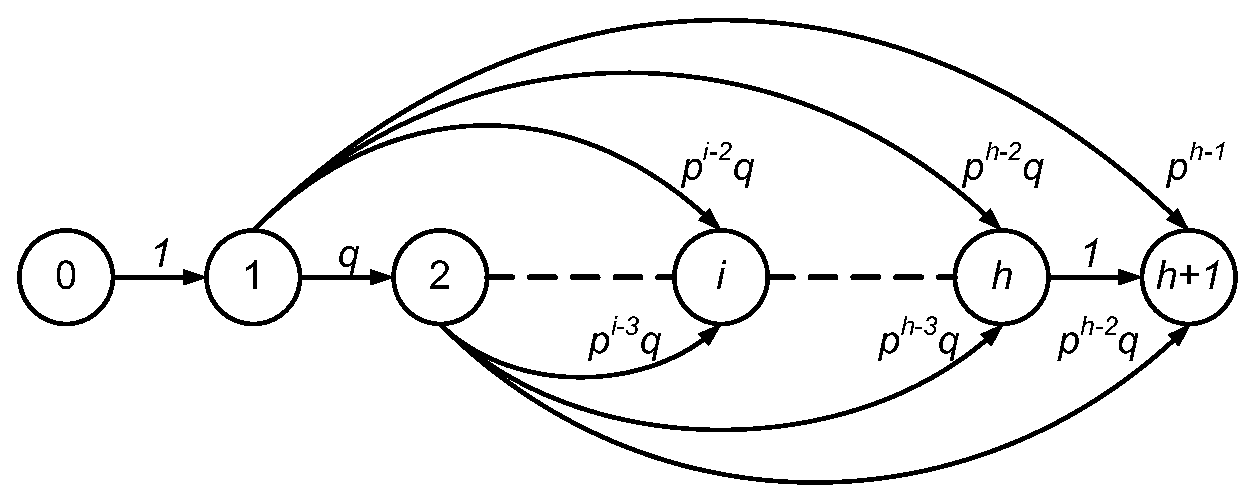
\includegraphics[width=0.35\textwidth]{Markov-SDHT-NoFail.eps}
     \caption{Markov Chain for Stealth DHT  without failures}
     \label{fig.sdht}}
\end{figure}

The correct next hop reference in a stealth node routing table may, by chance,
make as many prefix matches as possible. Thus, the Markov chain for Stealth DHT
model is the same as that of Pastry model for the rest of the states. In
particular, routing on a Stealth DHT is the same as routing on Pastry with a
network population equal to the number of service nodes. Fig.~\ref{fig.sdht}
shows the Markov chain for the Stealth DHT model with perfect routing. The
corresponding transition probabilities for are given as follows:

\[ p_{ji} = \left\{ \begin{array}{ll}
         0 & \mbox{if $j \le i$}\\
         1 & \mbox{if $i = 0$, $j = 1$}\\
         p^{j-i-1}q & \mbox{if $i \ge 1$, $i < j \le  h$} \\
         1   &  \mbox{if $i = h$, $j=h+1$}
         .\end{array} \right. \]

% AB: ergodic, is that correct?
To  obtain the expression for the average number of hops in the
Stealth DHT model with perfect routing where only stealth nodes send
messages ($H_{stealth}$) and with fraction of service nodes equal to
$r$ as, to modified the Markov chain the same way as we did for
Pastry in Section~\ref{mod.pastry}. Following such Markov chain
modification, the transition probability for the Stealth DHT perfect
routing model is now:
\[ {\bf P} = \left( \begin{array}{ccccccc}
0 & 1 & 0 & 0 & \cdots  0 & 0  & 0\\
0 & 0 & q & pq & \cdots &p^{h-2}q & p^{h-1}\\
0 & 0 & 0 &q & \cdots & p^{h-3}q & p^{h-2} \\
\cdots & \cdots & \cdots &\cdots & \cdots & \cdots & \cdots \\
0 & 0 & 0 &0 & \cdots & q & p \\
0 & 0 & 0 &0 & \cdots & 0 & 1 \\
1 & 0 & 0 &0 & \cdots & 0 & 0  \end{array} \right)\]

Note that $h  = log_{2^b}rN$, where $r$ is the fraction of service nodes in the
network. After some arithmetic operations, we obtain the steady state solution
of the corresponding linearly dependent equations as:
\[x_i = \left\{ \begin{array}{ll}
         x_0  & \mbox{if $i = 1,h+1$}\\
         qx_1 & \mbox{if $i = 2$} \\
         x_{i-1} & \mbox{if  $3 \le i \le h$} \end{array} \right. \]

Using this solution, we have $\pi_{h+1} = \frac{1}{(3+(h-1)q)}$, which yields
the mean recurrence time for state $h+1$ of the Stealth DHT routing model
($E[T_{h+1}]$) as :
\begin{equation}
\label{rT} E[T_{h+1}] = 3 + (h-1)q
\end{equation}
Subtracting 2 from Equation~(\ref{rT}), we obtain the average number of hops
for a Stealth DHT with perfect routing and that considers only stealth nodes to
send messages ($H_{stealth}$) as:
\begin{equation}
\label{Hs} H_{stealth} = (h-1)q + 1
\end{equation}

Due to the manner in which a stealth node functions, this never involves
sending a message to itself (which would often be the case for small Pastry
networks). The expression of the average number of hops for a Stealth DHT that
considers all nodes ($H_{SDHT}$) is:
\begin{eqnarray}
\nonumber
 H_{SDHT} &=& rH_{Pastry}  +  (1-r)H_{stealth} \\
\nonumber
 &=& rhq + (1-r)[(h-1)q + 1]\\
\label{complete_sdht}
 &=& hq  + (1-r)(1-q), \mbox{ $r > 0$}
\end{eqnarray}
where $h = log_{2^b}rN$ and $r$ is the fraction of service nodes.

Equation~(\ref{complete_sdht}) shows that the average number of hops for a
Stealth DHT is quite close to the average number of hops for Pastry when only
service nodes are considered. This is as expected, since stealth nodes do not
participate in routing and the first hop they make using their single row
routing table is no different from first hop of any service node using its
first row or a Pastry node in a network of the same size.

Similar to the case of Pastry, the perfect routing Stealth DHT model does not
portray an entirely realistic scenario. We therefore consider a Stealth DHT
model with routing imperfection in the following section.

\subsection{Model with Imperfect Routing}

The derivation of the Stealth DHT model with imperfect routing from the
associated perfect routing model simply follows the same procedures as that of
the equivalent Pastry models. For example, the closed form expression for
transition probabilities is easily obtained as:

\[ p_{ji} = \left\{ \begin{array}{ll}
         0 & \mbox{if $j < i$}\\
         1 & \mbox{if $i = 0$,  $j = 1$}\\
         p_f & \mbox{if $j = i$,  $i \neq 0, h+1 $}\\
         p^{j-i-1}qq_f & \mbox{if $ i \ge 1$, $ i < j \le h$} \\
         q_f & \mbox{if $i = h$, $j = h+1$}
         .\end{array} \right. \]

Using the same procedures as before, we get the expression for the
average number lookup hops for Stealth DHT model with probability of
routing failures $p_f$, and that considers only stealth nodes to
send messages ($H_{stealth}^f$) as:
\begin{equation}
\label{Hsf} H^f_{stealth} = \frac{(h-1)q + 1}{q_f}
\end{equation}
where $q_f = 1-p_f$.

The expression of the average number of hops for a Stealth DHT with imperfect
routing when considering all nodes is given as:
\begin{eqnarray}
\nonumber
 H_{SDHT}^f &=& rH_{Pastry}^f  +  (1-r)H_{stealth}^f \\
\label{complete_sdht_f}
 &=& \frac{hq  + (1-r)(1-q)}{q_f}
\end{eqnarray}

\subsection{Validation}
Simulations were carried out where 10,000 messages were sent from randomly
selected stealth nodes to randomly generated IDs within the address space. A
fixed network size totalling 1,000 nodes was considered, and the number of
service nodes was varied from 10 to 800, comprising 1\% to 80\% of the total
network respectively.

\begin{figure}[tb] \centering
     {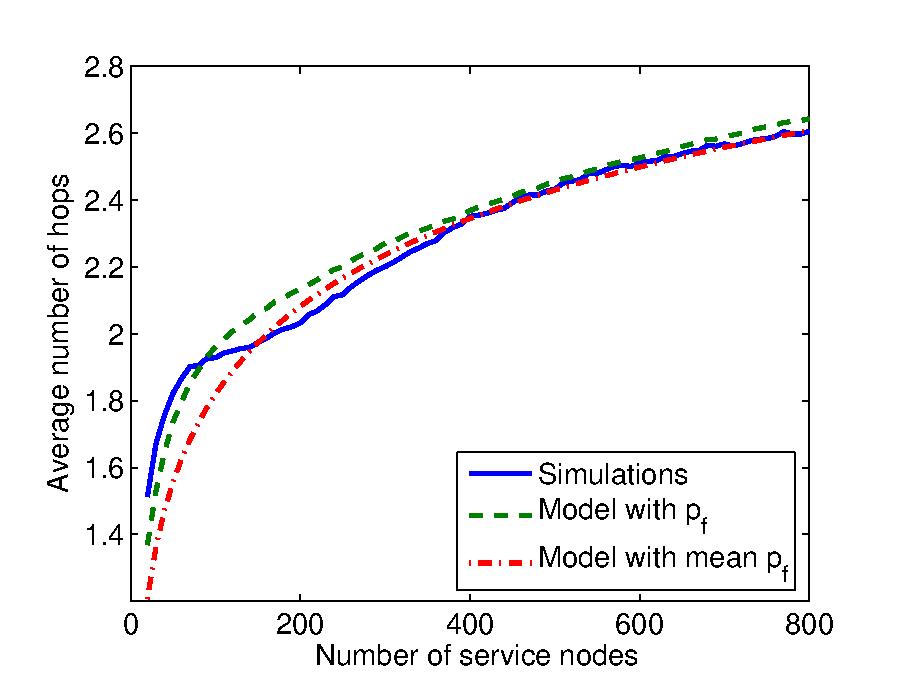
\includegraphics[width=0.4\textwidth]{val_stealth1.eps}
     %AB, the next line had $\overline{p_f}...$, but to make it fit the required font,
     % I have removed the overline. Hopefully thats still ok
     \caption{Validation of Stealth DHT with failures, p\subscript{f} = 0.1093}
     \label{fig.vstealth}}
\end{figure}

Fig.~\ref{fig.vstealth} shows the average number of hops of a Stealth DHT
obtained from models and simulations as a function of service nodes. We observe
a generally excellent agreement between the model and the simulations,
particularly for networks with large numbers of service nodes. However, the
model underestimates the simulations for both choices of probability for route
failures for small networks. This occurs in small networks because the routing
imperfection in stealth nodes severely alters the routing performance by
introducing randomness in choosing the next hop.
%We showed in
%\cite{Brampton06Stealth} that when compared to a random selection of nodes, a
%Stealth DHT using single row routing tables for stealth nodes provides superior
%performance. This is because that when a route fails, the message is forced to
%follow a non-optimal routing path, which increases the lookup length.
Additionally since most of route failures are observed at state 1 for small networks (see
Fig.~\ref{fig.fm}), a route failure at a stealth node makes it very likely for the route to fail at
the first service node as well. This is  because the service node will also use
the first row of its routing table. This, naturally makes the routing
performance worse.

\section{Conclusion}
\label{conc}

In this paper, we model the routing performance of  Pastry and its
corresponding Stealth DHT implementation and validate the models using
simulations of the protocols. We consider a perfect routing case in which
nodes' routing tables are assumed to be always full, as well a realistic case
where some cells in routing tables are often empty. Routing table imperfection
causes a lookup to follow a non-optimal routing path, which, through the
derived models in this paper, is shown to have an exponentially negative effect
on the routing performance of the protocols. We use simulations to demonstrate
that the models offer average routing performance that agree with the
simulation results very well. They can therefore be used instead of simulations
to quickly evaluate the protocols in a wide variety of experimental setups.

%In the future, we plan to extend the models in this paper to account for the
%effects of ``churn'' in DHT networks, where nodes leave and join the overlay
%rapidly. We also consider using the methodologies in this paper to model other
%DHT routing protocols, such as Chord, and their corresponding Stealth DHT
%implementations.

\small
\bibliographystyle{ipdps}
\bibliography{models}

\end{document}
